\documentclass[../review_2.tex]{subfiles}
\begin{document}

\chapter{Auswertung der erfassten Arbeitszeiten}\thispagestyle{fancy}

Mithilfe des  Zeiterfassungssystems Kimai können Arbeitszeiten der Teammitglieder erfasst werden. Dabei werden nicht nur der Beginn und das Ende der Bearbeitung einer Projektaufgabe von der Software aufgenommen, sondern es wird dieser auch eine passende Aktivitätskategorie und fakultativ ein kurzer Text hinzugefügt. Die verschiedenen Kategorien sind in diesem Projekt: 
\begin{itemize}
    \setlength{\parskip}{-0.2pt}
    \item Administration (z.B. Aktualisieren des Gantt-Diagramms)
    \item Entwurf (z.B. Erstellen des Klassendiagramms oder der Aktivitätsdiagramme)
    \item Dokumentation (z.B. Arbeiten am Review-Dokument)
    \item Implementierung (z.B. Ausprogrammieren einer konkreten Klasse)
    \item Installation (z.B. Herunterladen von DPDK)
    \item Meetings (z.B. Montagsmeeting mit dem Betreuer um 18:30 Uhr)
    \item Präsentationsvorbereitung (z.B. Erstellen der Präsentationsfolien)
    \item Recherche (z.B. Vergleichen verschiedener Maps durch Reports im Internet)
    \item Test (z.B. Ausführen von Unit Tests und anderen Tests)
\end{itemize}
Mithilfe dieses Tools kann somit jedes Teammitglied regelmäßig einen Überblick erhalten, was es wann wie lange für das Software-Projekt gemacht hat. \\
Am Ende jeder der drei Phasen (Planung- und Entwurf, Implementierung, Validierung) werden die vom Kimai erfassten Daten ausgewertet. Dies ermöglicht, Probleme zu identifizieren und so eventuell später aufkommende Komplikationen vorzubeugen. Falls sich somit in der Auswertung Probleme zeigen, werden Verbesserungsvorschläge und Gegenmaßnahmen entwickelt. \\
In diesem Kapitel werden die bisher erfassten Zeiten analysiert und in Diagrammen dargestellt. Diese Diagramme wurden automatisch aus den Daten einer Excel-Datei generiert. Diese Daten stimmen mit denen aus dem Kimai überein. %was bedeutet stand?

Wir haben den drei Phasen folgende Kalenderwochen zugeordnet:
\begin{itemize}
    \item Planungs- und Enturfsphase: KW 17 - KW 21
    \item Implementierungsphase: KW 22 - KW 24
    \item Validierungsphase: KW 25 - KW 29
\end{itemize}
Die Phasen werden in den folgenden Kapiteln einzeln ausgewertet und deren Ergebnisse am Ende verglichen.
\section{Planungs- und Entwurfsphase}

\begin{figure} [h]
   \centering
   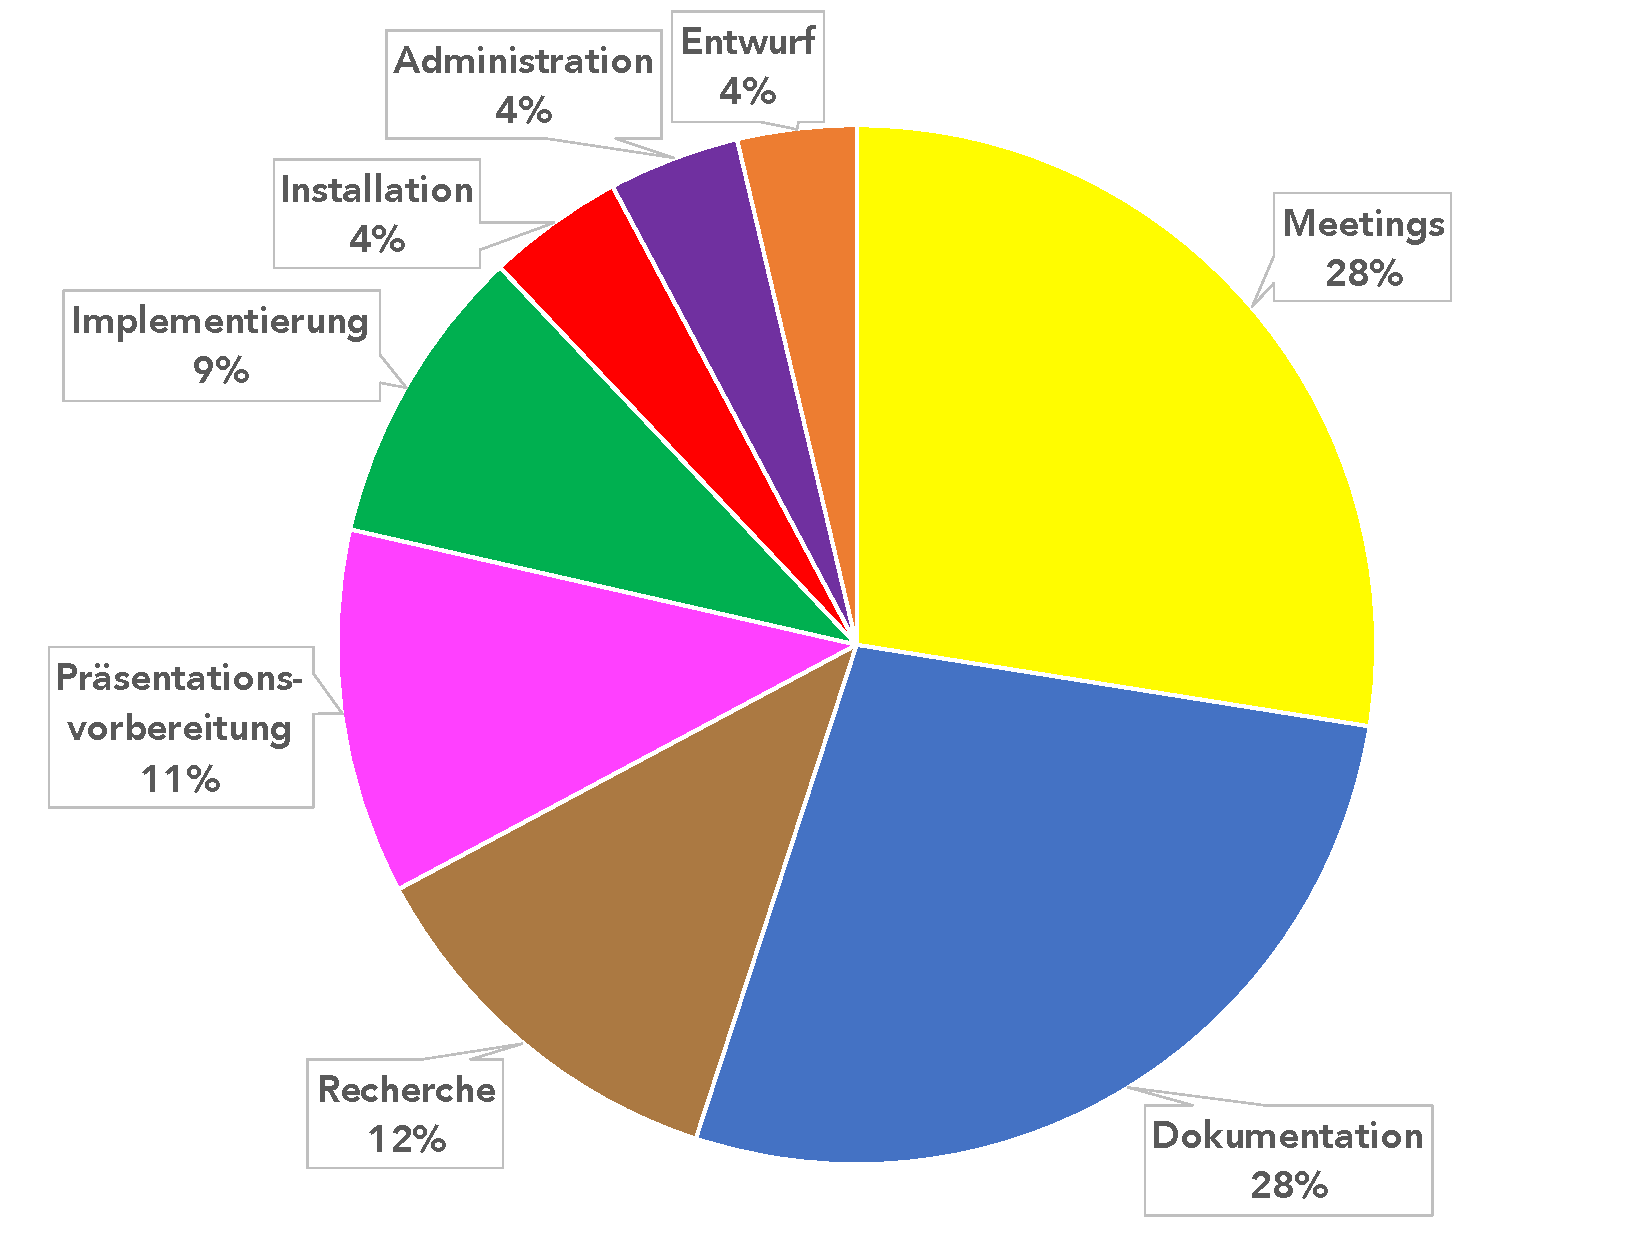
\includegraphics[width = \linewidth]{img/Kimai1.pdf}
    \caption{Planungs- und Entwurfsphase (KW 17-21): Anteile der Aufgabenkategorien an der insgesamt aufgebrachten Zeit}
    \label{kategorien}
\end{figure} 

Das Diagramm \ref{kategorien} zeigt, dass die Zeit in der Planungs- und Entwurfsphase vorwiegend für \textbf{Meetings} aufgewendet wurde. Der Grund dafür könnten die häufigen langen Diskussionen in den Meetings mit allen Teammitgliedern sein. Zudem wurde oft die gemeinsame Arbeit an Aufgaben ebenfalls als Meeting gebucht, auch wenn eine andere Kategorie besser gepasst hätte. Beispielsweise wurde das Klassendiagramm in den wöchentlichen Meetings gemeinsam entworfen. Diese Entwurfsaktivität wurde hier aber unter Meetings und nicht unter Entwurf verbucht. Lösungsideen sind, Meetings themenspezifischer zu buchen und diese nach Möglichkeit in kleineren Gruppen abzuhalten, falls die Themen nicht alle Mitglieder betreffen. Jedoch ist zu beachten, dass hierbei die Konsistenz gewahrt wird. Das bedeutet, dass die \glqq großen\grqq{} Meetings mit dem gesamten Team weiterhin unter Meetings verbucht werden müssen. Dies wurde sowohl bei einem Meeting als auch durch einen Eintrag im Wiki allen Teilnehmern des Projekts kommuniziert. Weiterhin könnten weniger bzw. kürzere Meetings gehalten werden und detaillierte Fragen direkt mit den zuständigen Personen geklärt werden. Dies dann entweder in einem eigenen Meeting oder über die Plattform Zulip.

Außerdem wurde mit 26\% viel Zeit für die Kategorie \textbf{Dokumentation} in Anspruch genommen. Ein möglicher Grund dafür ist, dass auch die Arbeit am Entwurf (z.B. am Klassen- oder Paketdiagramm) und die dazugehörige Entwurfsdokumentation nur unter der Kategorie Dokumentation, nicht aber unter der Kategorie Entwurf gebucht wurde. Daraus ergibt sich, dass das Team in Zukunft detaillierter buchen soll und die Kategorien womöglich angepasst werden muss.
Die für die \textbf{Recherche} aufgebrachte Zeit ist tendenziell verhältnismäßig und bedarf keiner Änderung.

Es fällt auf, dass für die \textbf{Vorbereitung} von Präsentationen  mit 11\% in dieser Projektphase vergleichsweise viel Zeit aufgewendet wurde. Dies resultiert daruas, dass jedes Teammitglied in der ersten Woche eine Präsentation zu verschiedenen Themen wie DoS-Angriffen oder DPDK gehalten hat und ein Template für Präsentationen erarbeitet werden musste. Im weiteren Verlauf des Projektes sollte dieser Anteil sinken, da dann nur noch eine Präsentation pro Phase gehalten werden muss. Zudem müssen womöglich weniger Grafiken für das Review erstellt werden und das Präsentationsdesign kann wiederverwendet werden.

Für die \textbf{Installation} sind 6\% der Zeit aufgebracht worden. Auch dieser Wert sollte im Verlauf sinken, weil ein Großteil der Installationen bereits erfolgt sind.

In der Planungs- und Entwurfsphase war der Zeitaufwand für die \textbf{Implementierung} sehr gering, was zu Beginn des Projektes allerdings kein Problem darstellt, da hier lediglich ein erster Prototyp mit stark reduziertem Funktionsumfang entwickelt wurde. Zudem kann es daraus resultieren, dass in dieser Phase mit der Implementierung lediglich zwei der acht Teammitglieder beauftragt waren. Es wird erwartet, dass mit Beginn der Implementierungsphase  der für die Implementierung erfasste Aufwand sprunghaft ansteigt.

Der geringe Anteil des \textbf{Administrationsaufwandes} ist positiv zu bewerten, weil er auf eine effiziente Planung und Verwaltung hinweist.

Die 3\% der erfassten Zeit, die der \textbf{Entwurf} in Anspruch genommen hat, sind zu wenig. Das ist wahrscheinlich darauf zurückzuführen, dass andere Kategorien für Arbeiten am Entwurf beim Buchen verwendet wurden, beispielsweise Dokumentation oder Meetings (Erklärung siehe oben).

\begin{figure} [h]
    \centering
    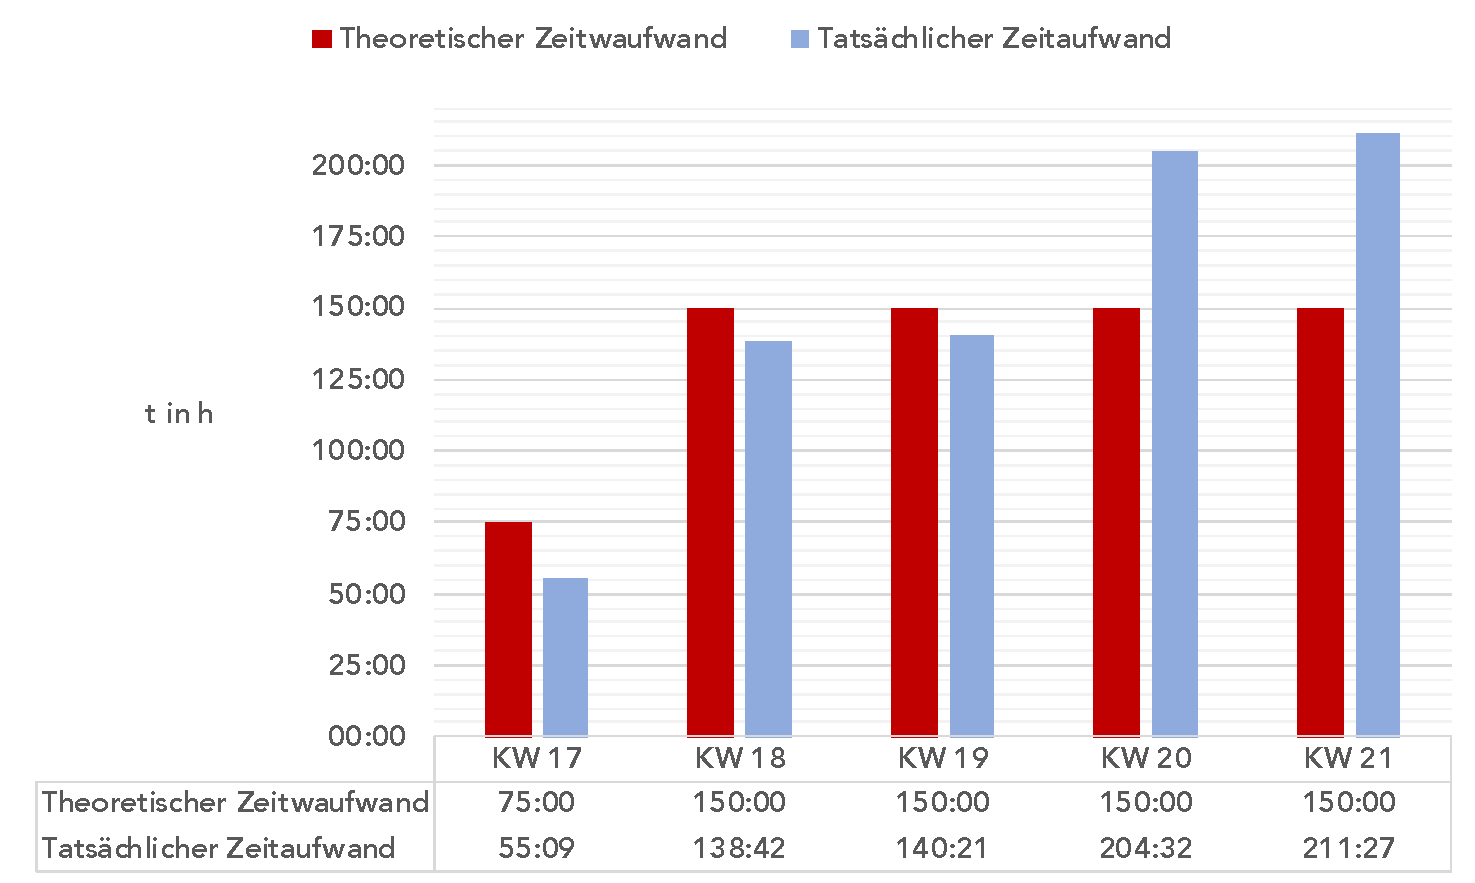
\includegraphics[width = \linewidth]{img/Kimai2.pdf}
    \caption{Planungs- und Entwurfsphase (KW 17-21): Vergleich des theoretischen Aufwands mit dem tatsächlichen Aufwand}
    \label{sollist}
\end{figure} 

Im Balkendiagramm in \ref{sollist} wird dem theoretischen Zeitaufwand pro Woche der tatsächliche Aufwand gegenübergestellt. Die hier angegebenen tatsächlichen Zeiten ergeben sich aus der Addition der wöchentlichen Zeiten aller Teammitglieder.
Während Informatiker und Ingenieurinformatiker für das Softwareprojekt acht Leistungspunkte angerechnet bekommen, beträgt diese Punktzahl bei Wirtschaftsinformatiker lediglich sechs. Deshalb wird als Richtwert für die aufzubringende Zeit pro Woche zwischen den Studiengängen unterschieden: Bei Informatikern und Ingenieurinformatikern beträgt dieser Wert 20 Wochenstunden, bei Wirtschaftsinformatikern dagegen nur 15 Wochenstunden.
Da das Team aus vier Informatikern, zwei Ingenieurinformatikern und zwei Wirtschaftsinformatikern besteht, beträgt der Soll-Wert pro Woche 150h.
\begin{equation*}
    2\cdot 20h + 4\cdot 20h + 2\cdot 15h = 150h
\end{equation*}
In Woche 17 liegt Soll-Wert nicht bei 150h, sondern bei 75h, da das Projekt erst am Donnerstag begonnen hat und somit diese Woche kürzer als die anderen war.

In dieser Kalenderwoche liegt der Ist-Wert fast 20h unter diesen 75h, nämlich bei 55h 9min. Dieses Defizit ist darin zu begründen, dass in dieser ersten Woche das Zeiterfassungssystem den Teammitgliedern noch nicht zur Verfügung stand. Deshalb mussten die Zeiten in der kommenden Woche nachgetragen werden, was jedoch nicht vom gesamten Team gemacht wurde.

In der Kalenderwoche 18 und der Kalenderwoche 19 liegt der tatsächliche Wert nur noch knapp unter den angestrebten 150 Stunden.

In den beiden letzten Wochen der ersten Phase werden diese 150h sogar stark übertroffen.
Somit lässt sich generell ein positiver Trend ablesen. Es wird jedoch erwartet, dass der in der kommenden Projektphase aufgebrachte Aufwand nicht weiter stark ansteigen wird, da es neben dem Softwareprojekt noch zahlreiche andere Aufgaben für das Studium zu erledigen gibt. Somit ist es für die meisten Studierende kaum möglich, mehr als 20 bis 30 Stunden für dieses Projekt in Anspruch zu nehmen.

\begin{figure} [h]
    \centering
    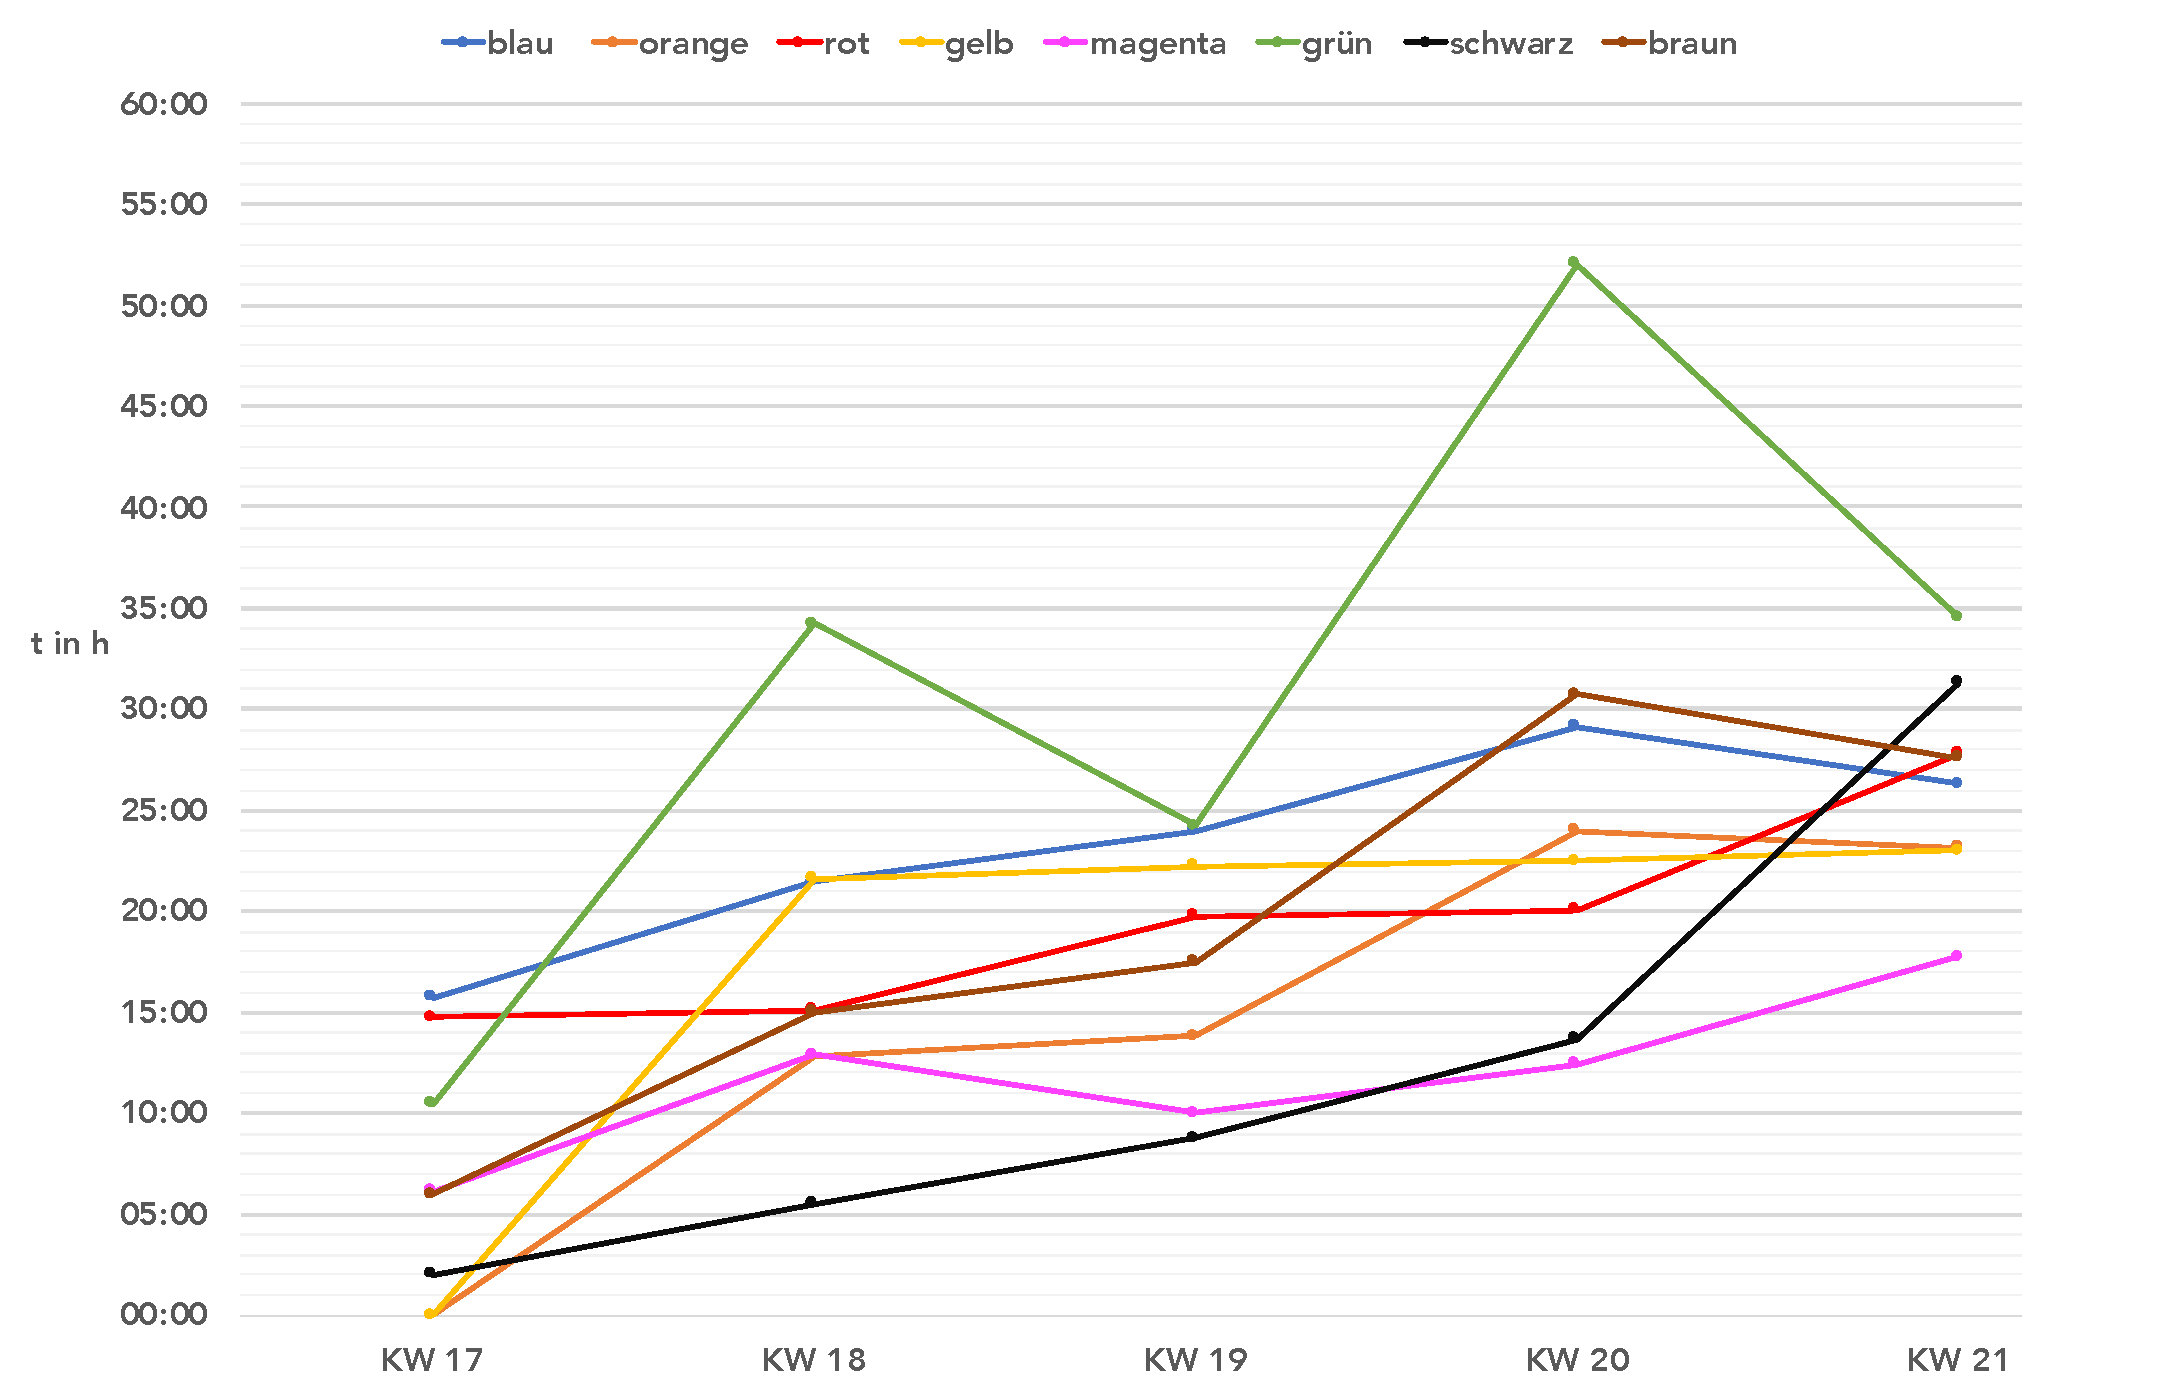
\includegraphics[width = \linewidth]{img/Kimai3.pdf}
    \caption{Planungs- und Entwurfsphase (KW 17-21): Zeitaufwand der einzelnen Teammitglieder}
    \label{teammitglieder}
\end{figure} 

\begin{figure} [h]
    \centering
    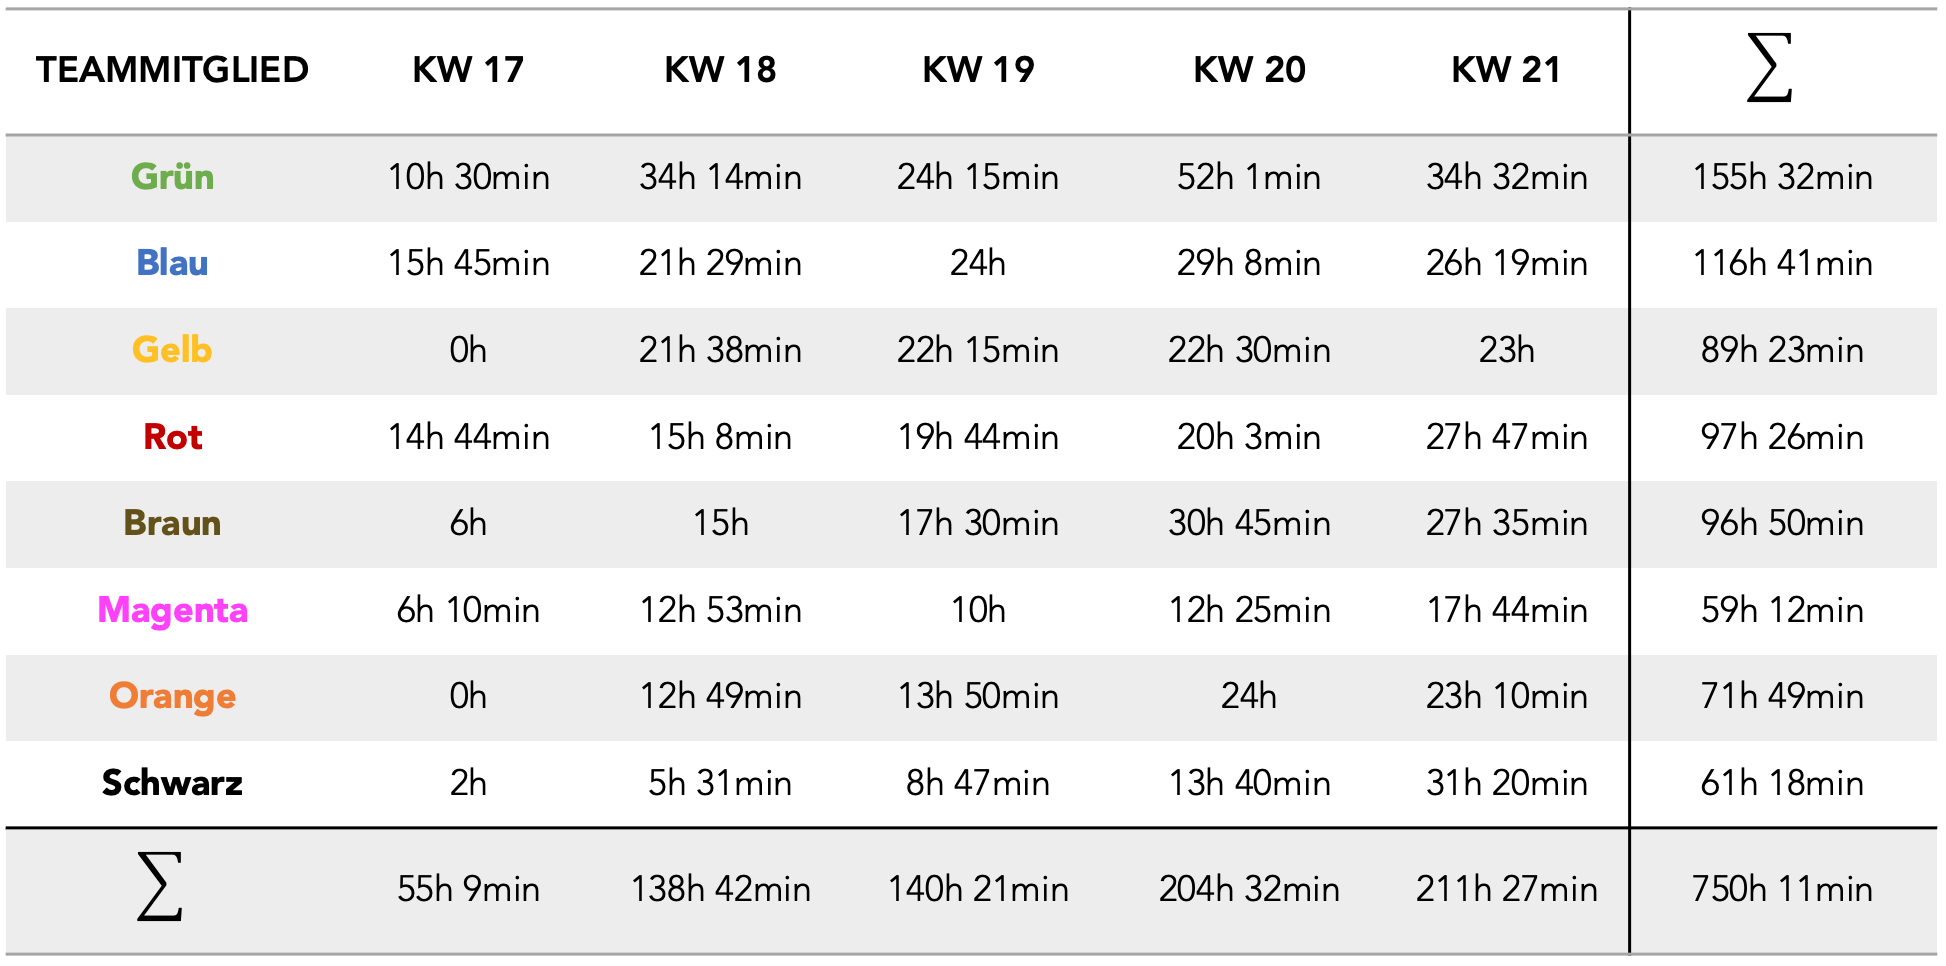
\includegraphics[width = \linewidth]{img/Kimai4.png}
    \caption{Planungs- und Entwurfsphase (KW 17-21): Tabelle zum Zeitaufwand der einzelnen Teammitglieder}
    \label{teammitglieder2}
\end{figure} 

Den Abbildungen \ref{teammitglieder} und \ref{teammitglieder2} ist zu entnehmen, dass teilweise große Unterschiede zwischen den Teammitgliedern in Bezug auf die wöchentlich aufgebrachten Stunden für das Softwareprojekt bestehen. \footnote{\noindent Jede Linienfarbe in einem Projektmitglied zugeordnet. Auf die Beschriftung der einzelnen Linien wurde jedoch verzichtet, um die Anonymität der einzelnen Personen zu wahren.}
Aus dem Diagramm geht hervor, dass in Kalenderwoche 17 noch nicht jeder seine Arbeitszeiten in das Kimai eingetragen hat, da es zu diesem Zeitpunkt Ihnen noch nicht zur Verfügung stand und sie diese hätten nachtragen müssen. Somit liegt bei zwei Personen der Wert in KW17 bei 0.
Es ist ein positiver Trend zu sehen, was auch in der Abbildung \ref{sollist} deutlich wurde.
Es ist hervorzuheben, dass einzelne Mitglieder weit über 20 Stunden pro Woche für das Softwareprojekt aufwenden. In der Kalenderwoche 20 liegt diese beispielsweise bei einem Teammitglied über 52 Stunden.


\section{Implementierungsphase}
\begin{figure} [h]
    \centering
    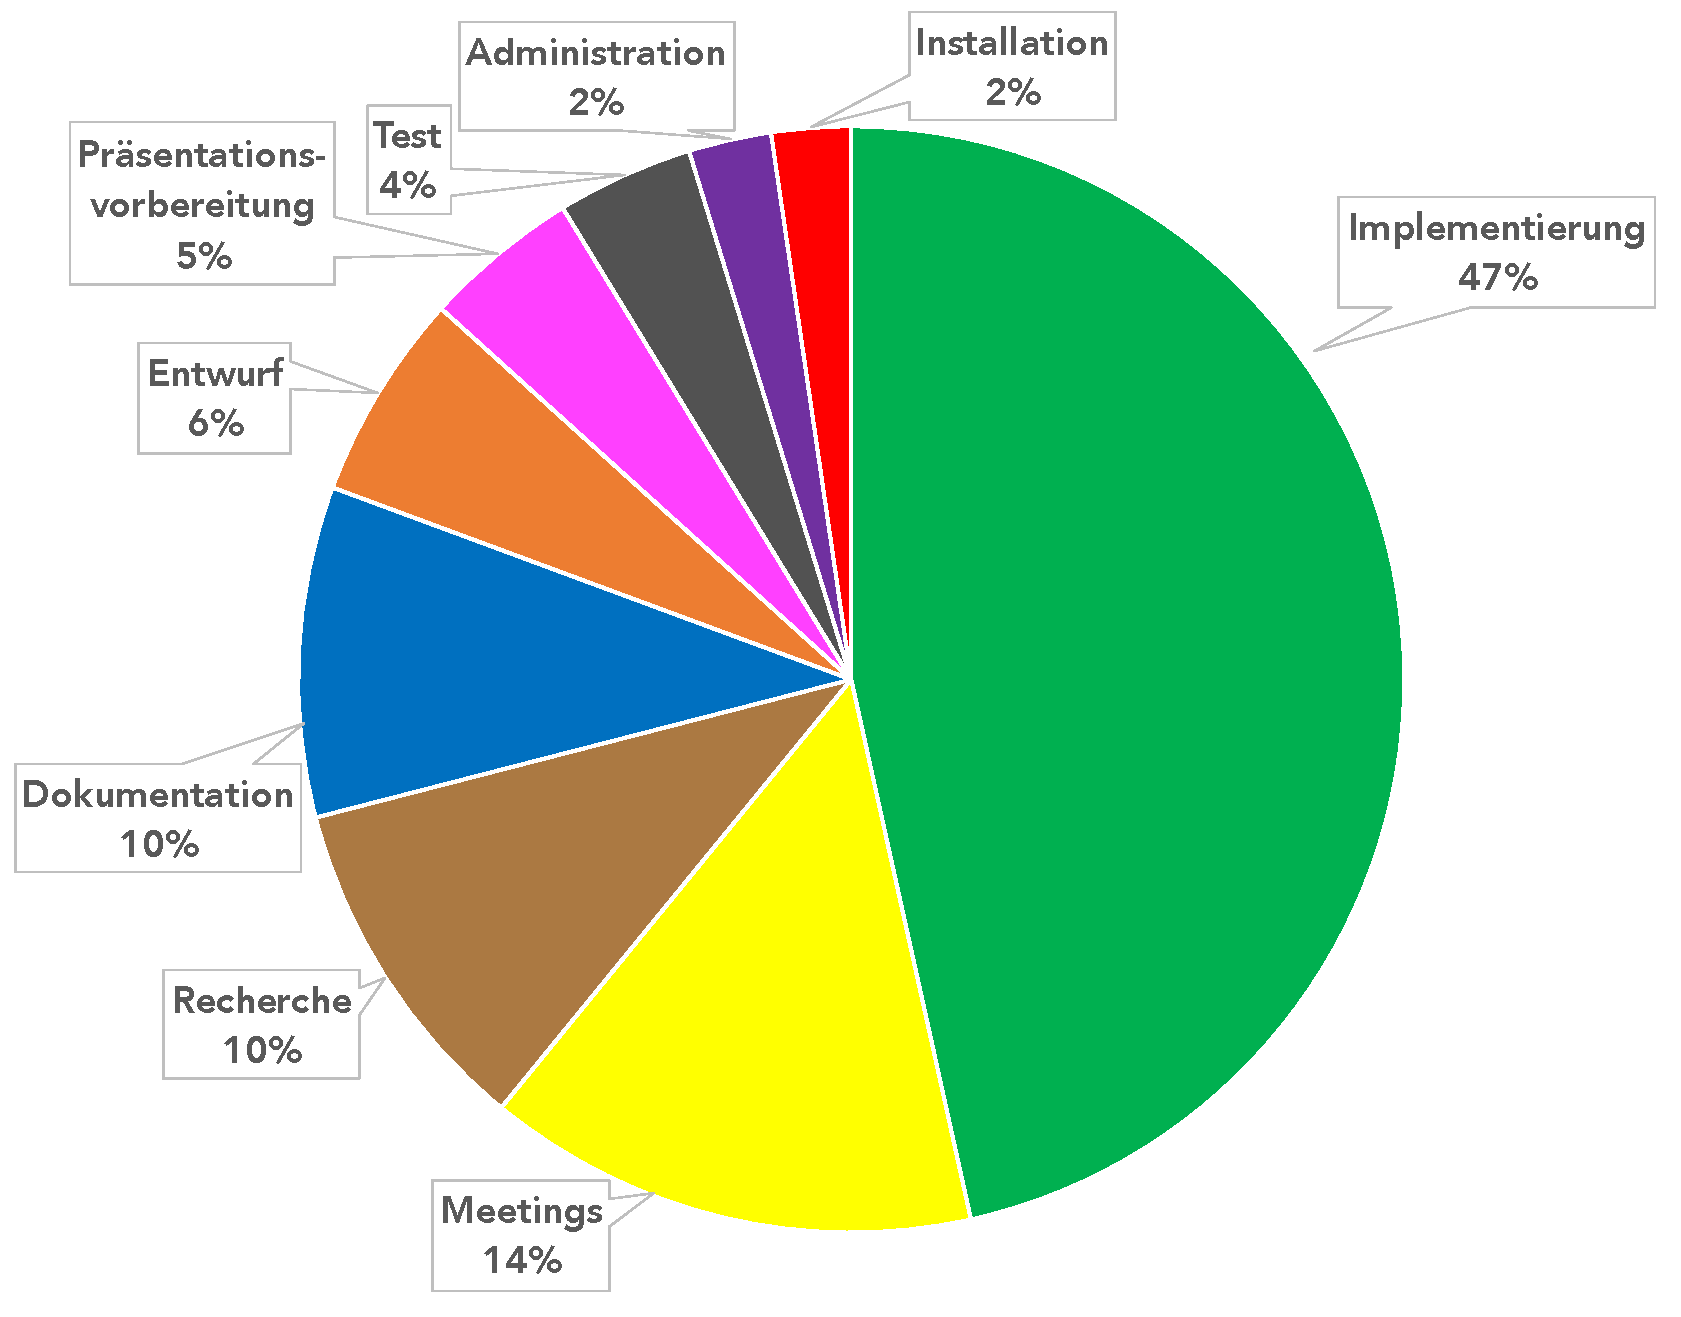
\includegraphics[width = \linewidth]{img/kimai5.pdf}
    \caption{Implementierungsphase (KW 22-24): Anteile der Aufgabenkategorien an der insgesamt aufgebrachten Zeit}
    \label{kimai5}
\end{figure} 
Wie in Abbildung \ref{kimai5} zu sehen ist, wurde fast die Hälfte der Zeit dieser Projektphase für die \textbf{Implementierung} verwendet. Dieser Anteil ist durchaus angemessen, weil in der Implementierungsphase der größte Teil des Systems programmiert werden soll.

\textbf{Meetings} stellen mit 14\% die zweithäufigste Kategorie dar. Diese Größe bedarf nicht zwangsläufig einer Änderung, da die Meetings in dieser Phase lediglich wichtige Themen umfasst haben und so kurz wie möglich gehalten wurden. Außerdem bleibt zu erwähnen, dass in zwei Meetings ein Code-Review durchgeführt wurde, wodurch alle Teammitglieder voneinander lernen konnten und das System insgesamt sowie von anderen entwickelte Komponenten besser verstanden werden konnten.

Die Kategorien \textbf{Recherche} und \textbf{Dokumentation} nahmen beide ein Zehntel der insgesamt aufgebrachten Zeit in Anspruch und gehen somit mit einem angemessenen Anteil in das Projekt ein.

Die 6\%, die dem \textbf{Entwurf} zugeordnet werden können, sind relativ wenig. Möglicherweise wurde für diese Kategorie aufgebrachte Zeit auch in andere Kategorien wie Dokumentation oder Implementierung gebucht.

Positiv zu bewerten ist, dass die restlichen Kategorien, also \textbf{Präsentationsvorbereitung}, \textbf{Test}, \textbf{Administration} und \textbf{Installation}, höchstens 5\% der Zeit in Anspruch genommen haben. Trotzdem ist es wichtig, dass die den Tests zugeordnete Zeit in der kommenden Validierungsphase sprunghaft ansteigt. In der Implementierungsphase hat es sich dabei vor allem um Unit-Tests gehandelt, die für die gesamte Validierung nicht ausreichen 
werden.

\begin{figure} [h]
    \centering
    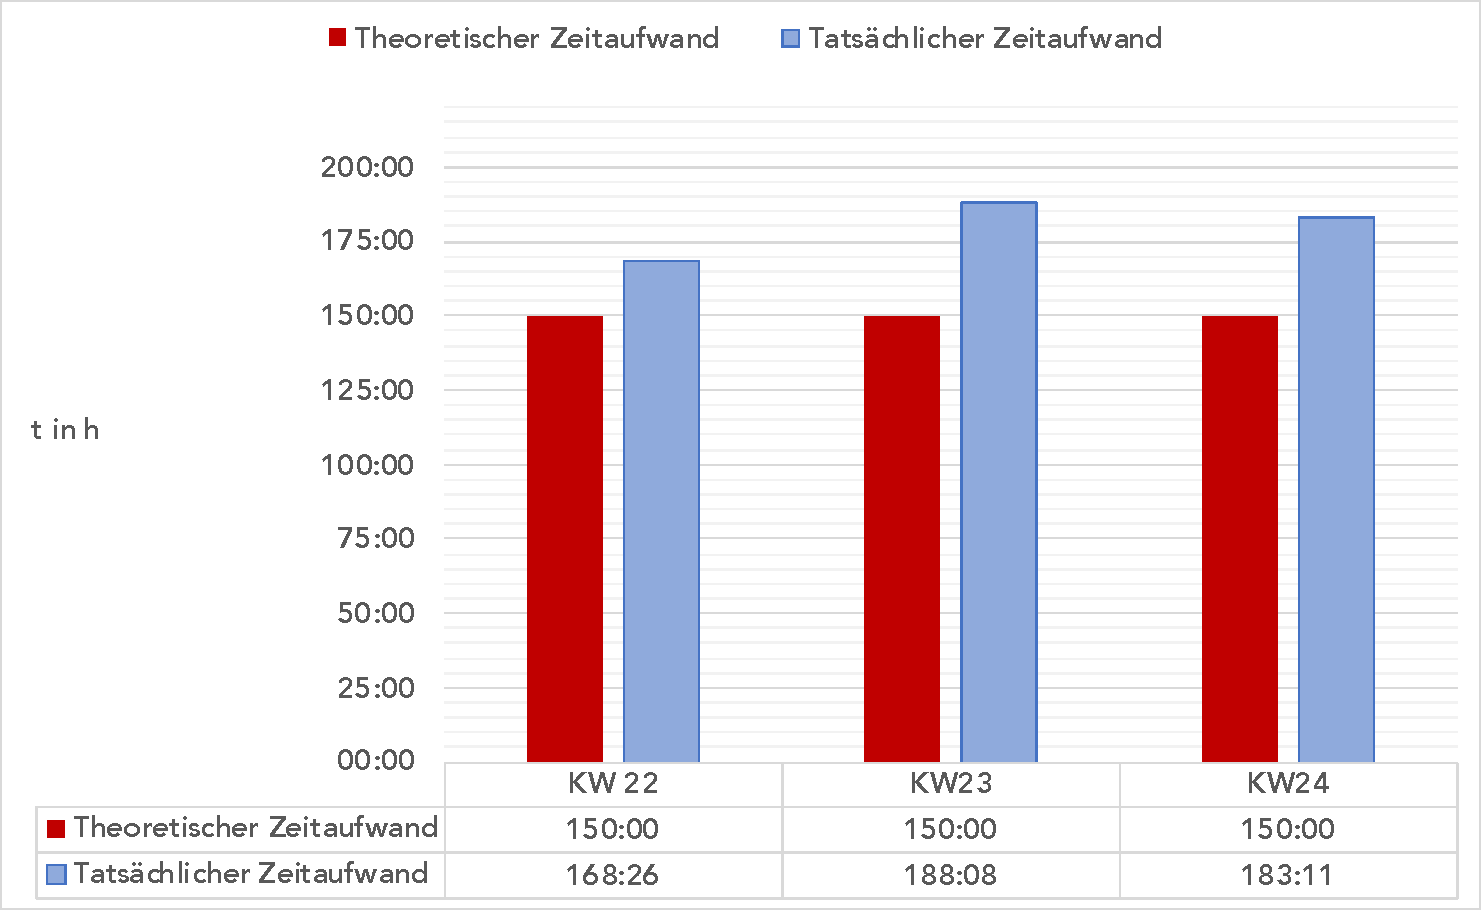
\includegraphics[width = \linewidth]{img/kimai7.pdf}
    \caption{Implementierungsphase (KW 22-24): Vergleich des theoretischen Aufwands mit dem tatsächlichen Aufwand}
    \label{kimai7}
\end{figure} 
Abbildung \ref{kimai7} macht deutlich, dass in jeder einzelnen Woche der Implementierungsphase (KW 22 - 24) der tatsächliche Zeitaufwand über dem theoretischen Zeitaufwand lag. Die vorgegebenen 150h Stunden Zeitaufwand pro Woche wurden in der Kalenderwoche 23 sogar um über 38h überschritten. Wenn man diese 38h durch die Anzahl der Teammitglieder teilt, die bei acht liegt, wird deutlich, dass in dieser Woche im Durchschnitt jedes Teammitglied 4h und 45min mehr Zeit für das Softwareprojekt aufgewendet hat als vorgegeben.
\begin{figure} [h]
    \centering
    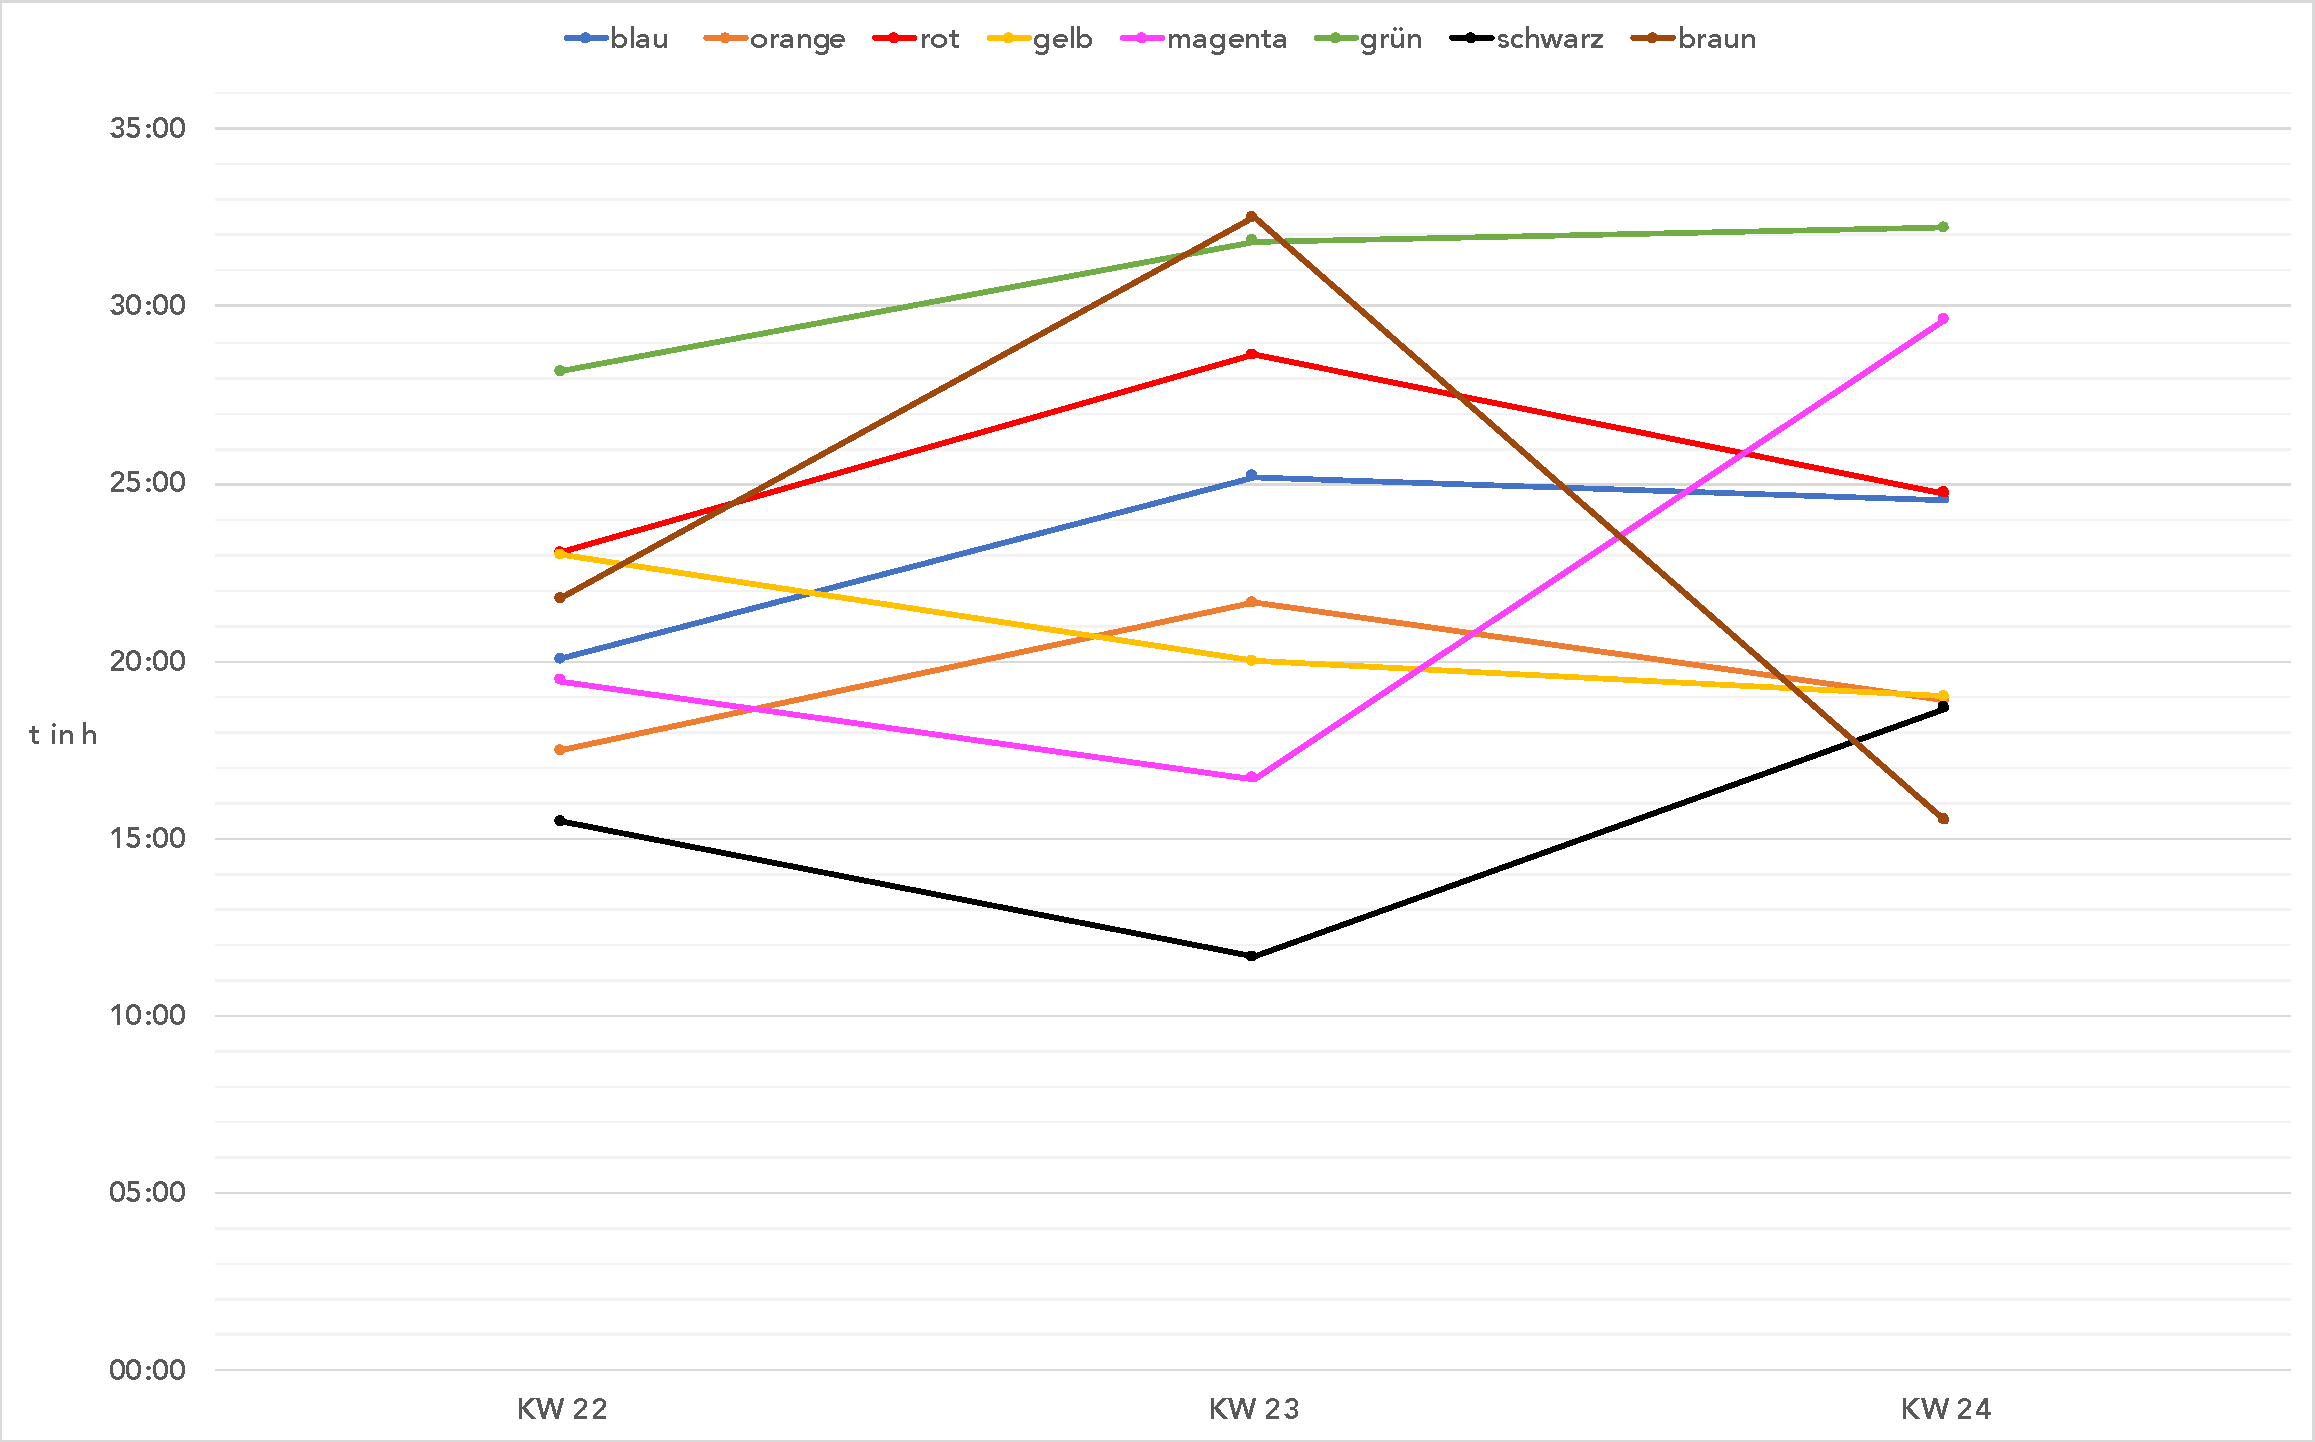
\includegraphics[width = \linewidth]{img/kimai9.pdf}
    \caption{Implementierungsphase (KW 22-24): Zeitaufwand der einzelnen Teammitglieder}
    \label{kimai9}
\end{figure} 

Aus Abbildung \ref{kimai9} lässt sich grundsätzlich kein starker Anstieg der Zeit, die jeder einzelne Beteiligte für das Softwareprojekt aufgewendet hat, erkennen. Bei sechs der acht Teammitglieder liegt ihr persönliches Maximum in diesem Zeitraum in KW 23. Hier liegt auch der Punkt, mit dem größten Wert in der Implementierungsphase. Der dazugehörige Wert beträgt 32h 30min (vgl. Abb. \ref{kimai11}).
Bei einigen Teammitglieder kann erkannt werden, dass die empfohlene Zeit von 15 bzw. 20 Stunden in einzelnen Fällen unterschritten wird. Üblicherweise wird auf die gesamte Zeit bezogen der Soll-Wert allerdings erfüllt, was man auch in Abbildung \ref{kimai7} erkennen kann.


\begin{figure} [h]
    \centering
    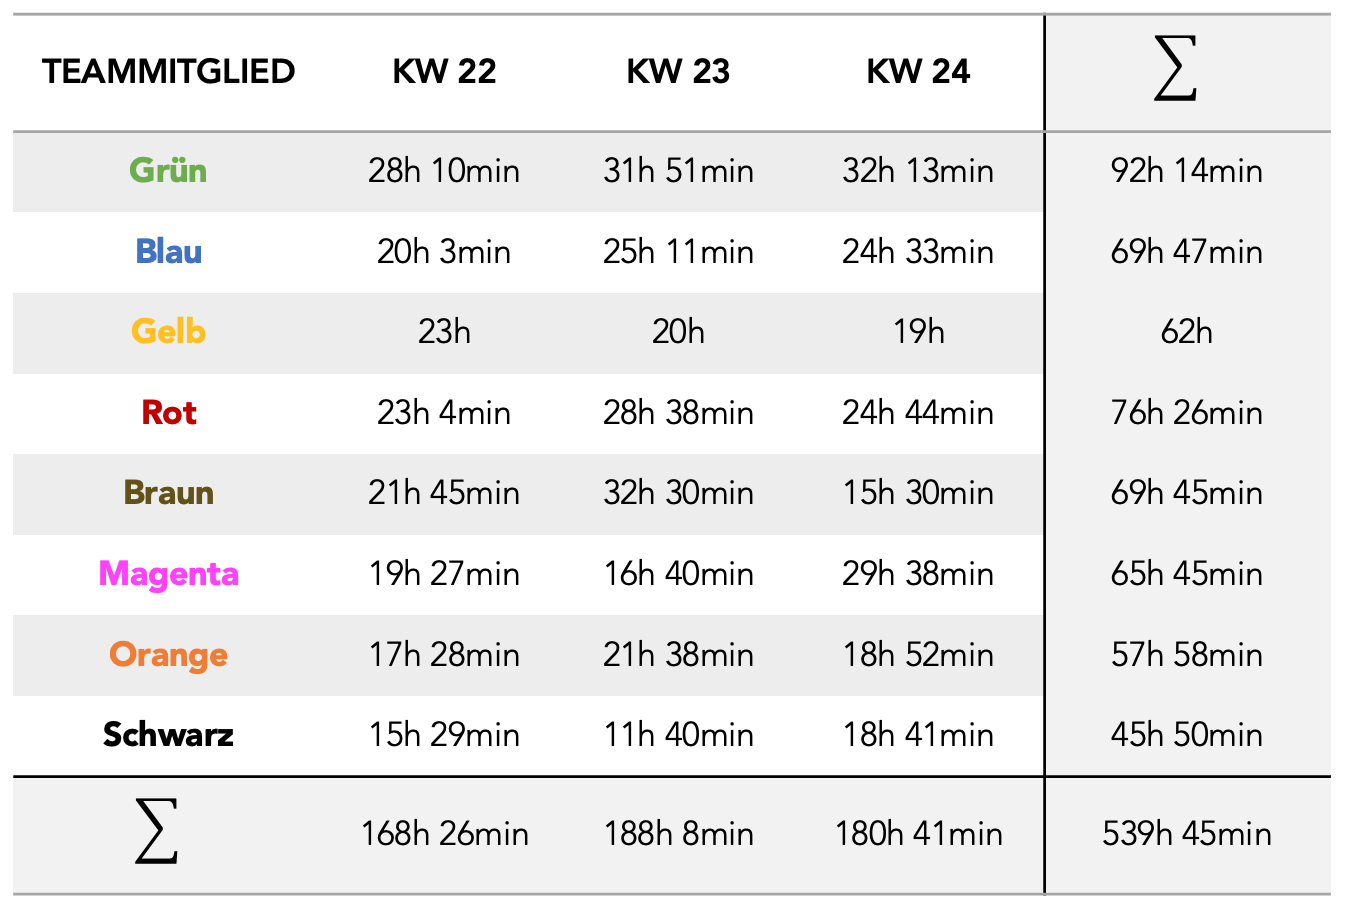
\includegraphics[width = 0.8\linewidth]{img/kimai11.png}
    \caption{Implementierungsphase (KW 22-24): Tabelle mit den erfassten Zeiten}
    \label{kimai11}
\end{figure} 

\section{Vergleich der Projektphasen}
\begin{figure} [h]
    \centering
    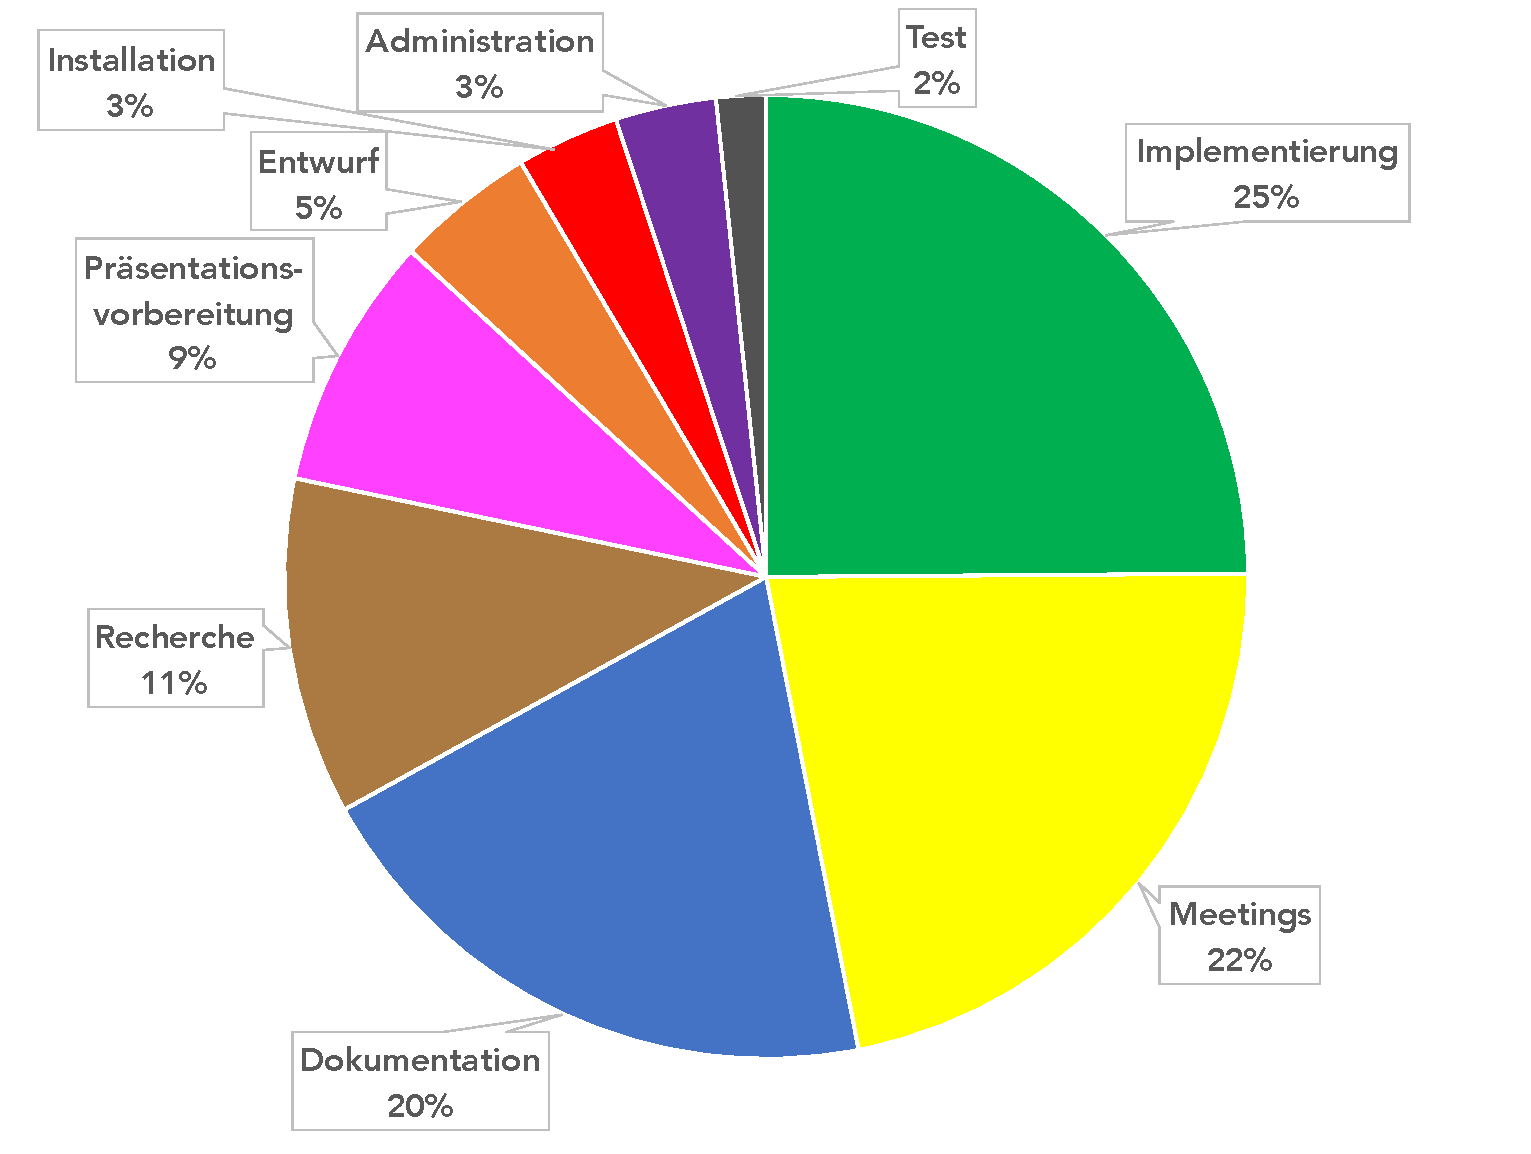
\includegraphics[width = 0.8\linewidth]{img/kimai6.pdf}
    \caption{Planungs- und Entwurfsphase und Implementierungsphase (KW 17-24): Anteile der Aufgabenkategorien an der insgesamt aufgebrachten Zeit}
    \label{kimai6}
\end{figure} 
In Abbildung \ref{kimai7} wird die Verteilung der Kategorien bezogen auf den gesamten Projektzeitraum dargestellt.

Bei einem Vergleich der Anteile der Kategorien an der insgesamt aufgebrachten Zeit zwischen Planungs- und Entwurfsphase und Implementierungsphase fällt als erstes auf, dass sich die für die \textbf{Implementierung} aufgebrachte Zeit vervielfacht hat. Dieser sprunghafte Anstieg wurde auch prognostiziert, weil die Implementierung in der ersten Phase lediglich einen ersten Prototyp umfasste und der zentrale Bestandteil der jetzt abgeschlossenen Phase ist.

Weiterhin ist der Anteil der \textbf{Meetings} von 29 auf 14\% gesunken. Da dieser Anteil im ersten Abschnitt des Softwareprojekts viel zu hoch war und schließlich auf einen adäquaten Wert gesenkt werden konnte, kann geschlussfolgert werden, dass die richtigen Maßnahmen getroffen wurden. So wurden Diskussionen, die nicht alle Teammitglieder betroffen haben, von den wöchentlichen Treffen in kleinere Gruppen verlagert und dann in der entsprechenden Kategorie themenbezogen gebucht.

Die \textbf{Dokumentation} hat während der Implementierungsphase ebenfalls weniger Zeit in Anspruch genommen als in der Planungs- und Entwurfsphase. Das umfassende Reviewdokument der ersten Phase, bestehend aus dem Pflichtenheft und einer Entwurfsdokumentation, stellte im ersten Monat des Projekts eine der Hauptaufgaben dar, während ihm in dieser Phase lediglich eine mittelhohe Priorität zugeordnet wurde.

Der \textbf{Rechercheaufwand} ist leicht gesunken, da sich zu Beginn des Projekts besonders viel Wissen angeeignet werden musste, welches im Laufe des Projekts dann zunehmen angewendet werden musste. Da fast alle Teammitglieder zu Beginn des Projekts recht unerfahren waren, scheinen die 11\% der im gesamten Projektzeitraum aufgebrachten Zeit ein geeigneter Anteil zu sein.

Insgesamt wurden 9\% der Zeit für die Vorbereitung von \textbf{Präsentationen} verwendet, was ebenfalls positiv zu bewerten ist. An dieser Stelle muss angemerkt werden, dass die Zeiterfassung der Implementierungsphase lediglich die Zeiten bis KW 24 umfasst, wodurch die letzten drei Tage vor der Präsentation nicht abgedeckt wurden. In dieser Zeit wird vermutlich noch eine nicht zu vernachlässigende Menge an Zeit für die Vorbereitung des zweiten Reviews investiert werden. Aus diesem Grund und weil jedes Teammitglied in der ersten Woche des Projekts eine Präsentation zu einem bestimmten Thema ausgearbeitet hat, ist der Wert von 11\% auf 5\% zurückgegangen.

Der \textbf{Entwurf} umfasste insgesamt 5\% der Zeit und wurde in beiden Phasen tendenziell zu wenig beziehungsweise in anderen, ähnlichen Kategorien erfasst.

Für die \textbf{Installation} musste sogar in der ersten Phase nur 5\% der Zeit verwendet werden. In der Implementierungsphase sank dieser Anteil auf 2\%. Da fast alle benötigten Komponenten bereits installiert sein sollten, lässt sich vermuten, dass der Anteil dieser Kategorie in der letzten Projektphase weiter gegen null geht.

Der \textbf{Administrationsaufwand} konnte schon in der ersten Phase des Projekts gering gehalten werden und ging auch in der Implementierungsphase in einem geeigneten Maß ein.

In der zweiten Phase hat sich der \textbf{Testaufwand} von 2 auf 4\% verdoppelt. Das zeigt, dass die Projektverlauf zunehmende Bedeutung des Testens erkannt wurde. Wichtig ist allerdings, dass beim Testen in der nächsten Phase ein sprunghafter Anstieg ähnlich wie bei der Implementierung zwischen erster und zweiter Phase zu erkennen ist.

\begin{figure} [h]
    \centering
    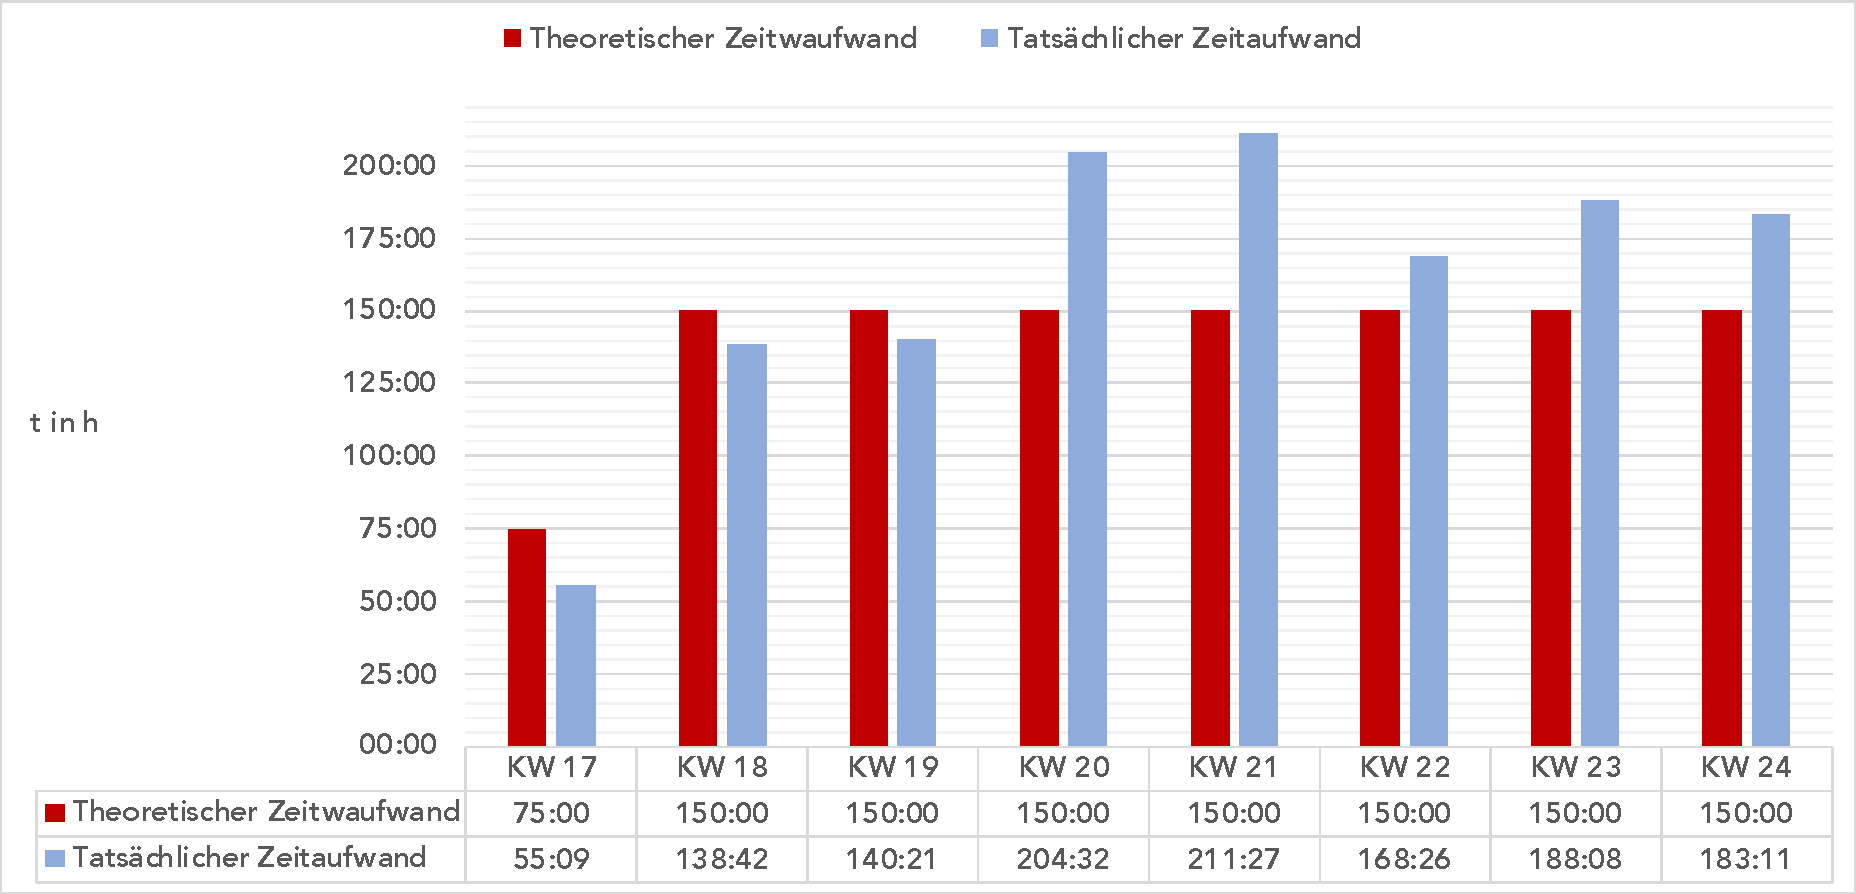
\includegraphics[width = \linewidth]{img/kimai8.pdf}
    \caption{Planungs- und Entwurfsphase und Implementierungsphase (KW 17-24): Vergleich des theoretischen Aufwands mit dem tatsächlichen Aufwand}
    \label{kimai8}
\end{figure} 
Folgendes lässt sich in Abbildung \ref{kimai8} erkennen:
Während in den ersten drei Wochen des Softwareprojekts (KW 17-18) der tatsächliche Zeitaufwand noch leicht unter dem theoretischen Wert liegt, ändert sich dies in den darauffolgenden Wochen dahingehend, dass der tatsächliche Zeitaufwand den theoretischen (zum Teil stark) übersteigt.
Die Feststellung, dass mehr Zeit aufgewendet wird bzw. werden muss als vorgegeben,  stimmt mit der Aufwandsschätzung aus dem ersten Reviewdokument überein.
Denn wenn die theoretischen Werte aller bisherigen Wochen (KW 17-24) aufaddiert werden, ergibt sich ein Wert von 1289h 56min (vgl. Abb. \ref{kimai12}). Diesem stehen 1125h entgegen:
\begin{align*}
    1 \cdot 75h+7 \cdot 150h= 1125h
\end{align*}
In der ersten Aufwandssschätzung schätzten wir den Aufwand des gesamten Projekts auf 2107h.
Würden wir in den kommenden Wochen (KW 25-29) \glqq lediglich\grqq{} den theoretische berechnete Zeit brauchen, wären das zu den bisher benötigten 1289h 56min noch 675h, also insgesamt 1964h 56min. Dieser Wert kommt dem Schätzwert aus der Aufwandsschätzung sehr nahe.
\begin {align*}
4 \cdot 150h + 1 \cdot 75h = 675h
\end{align*}

\begin{figure} [h]
    \centering
    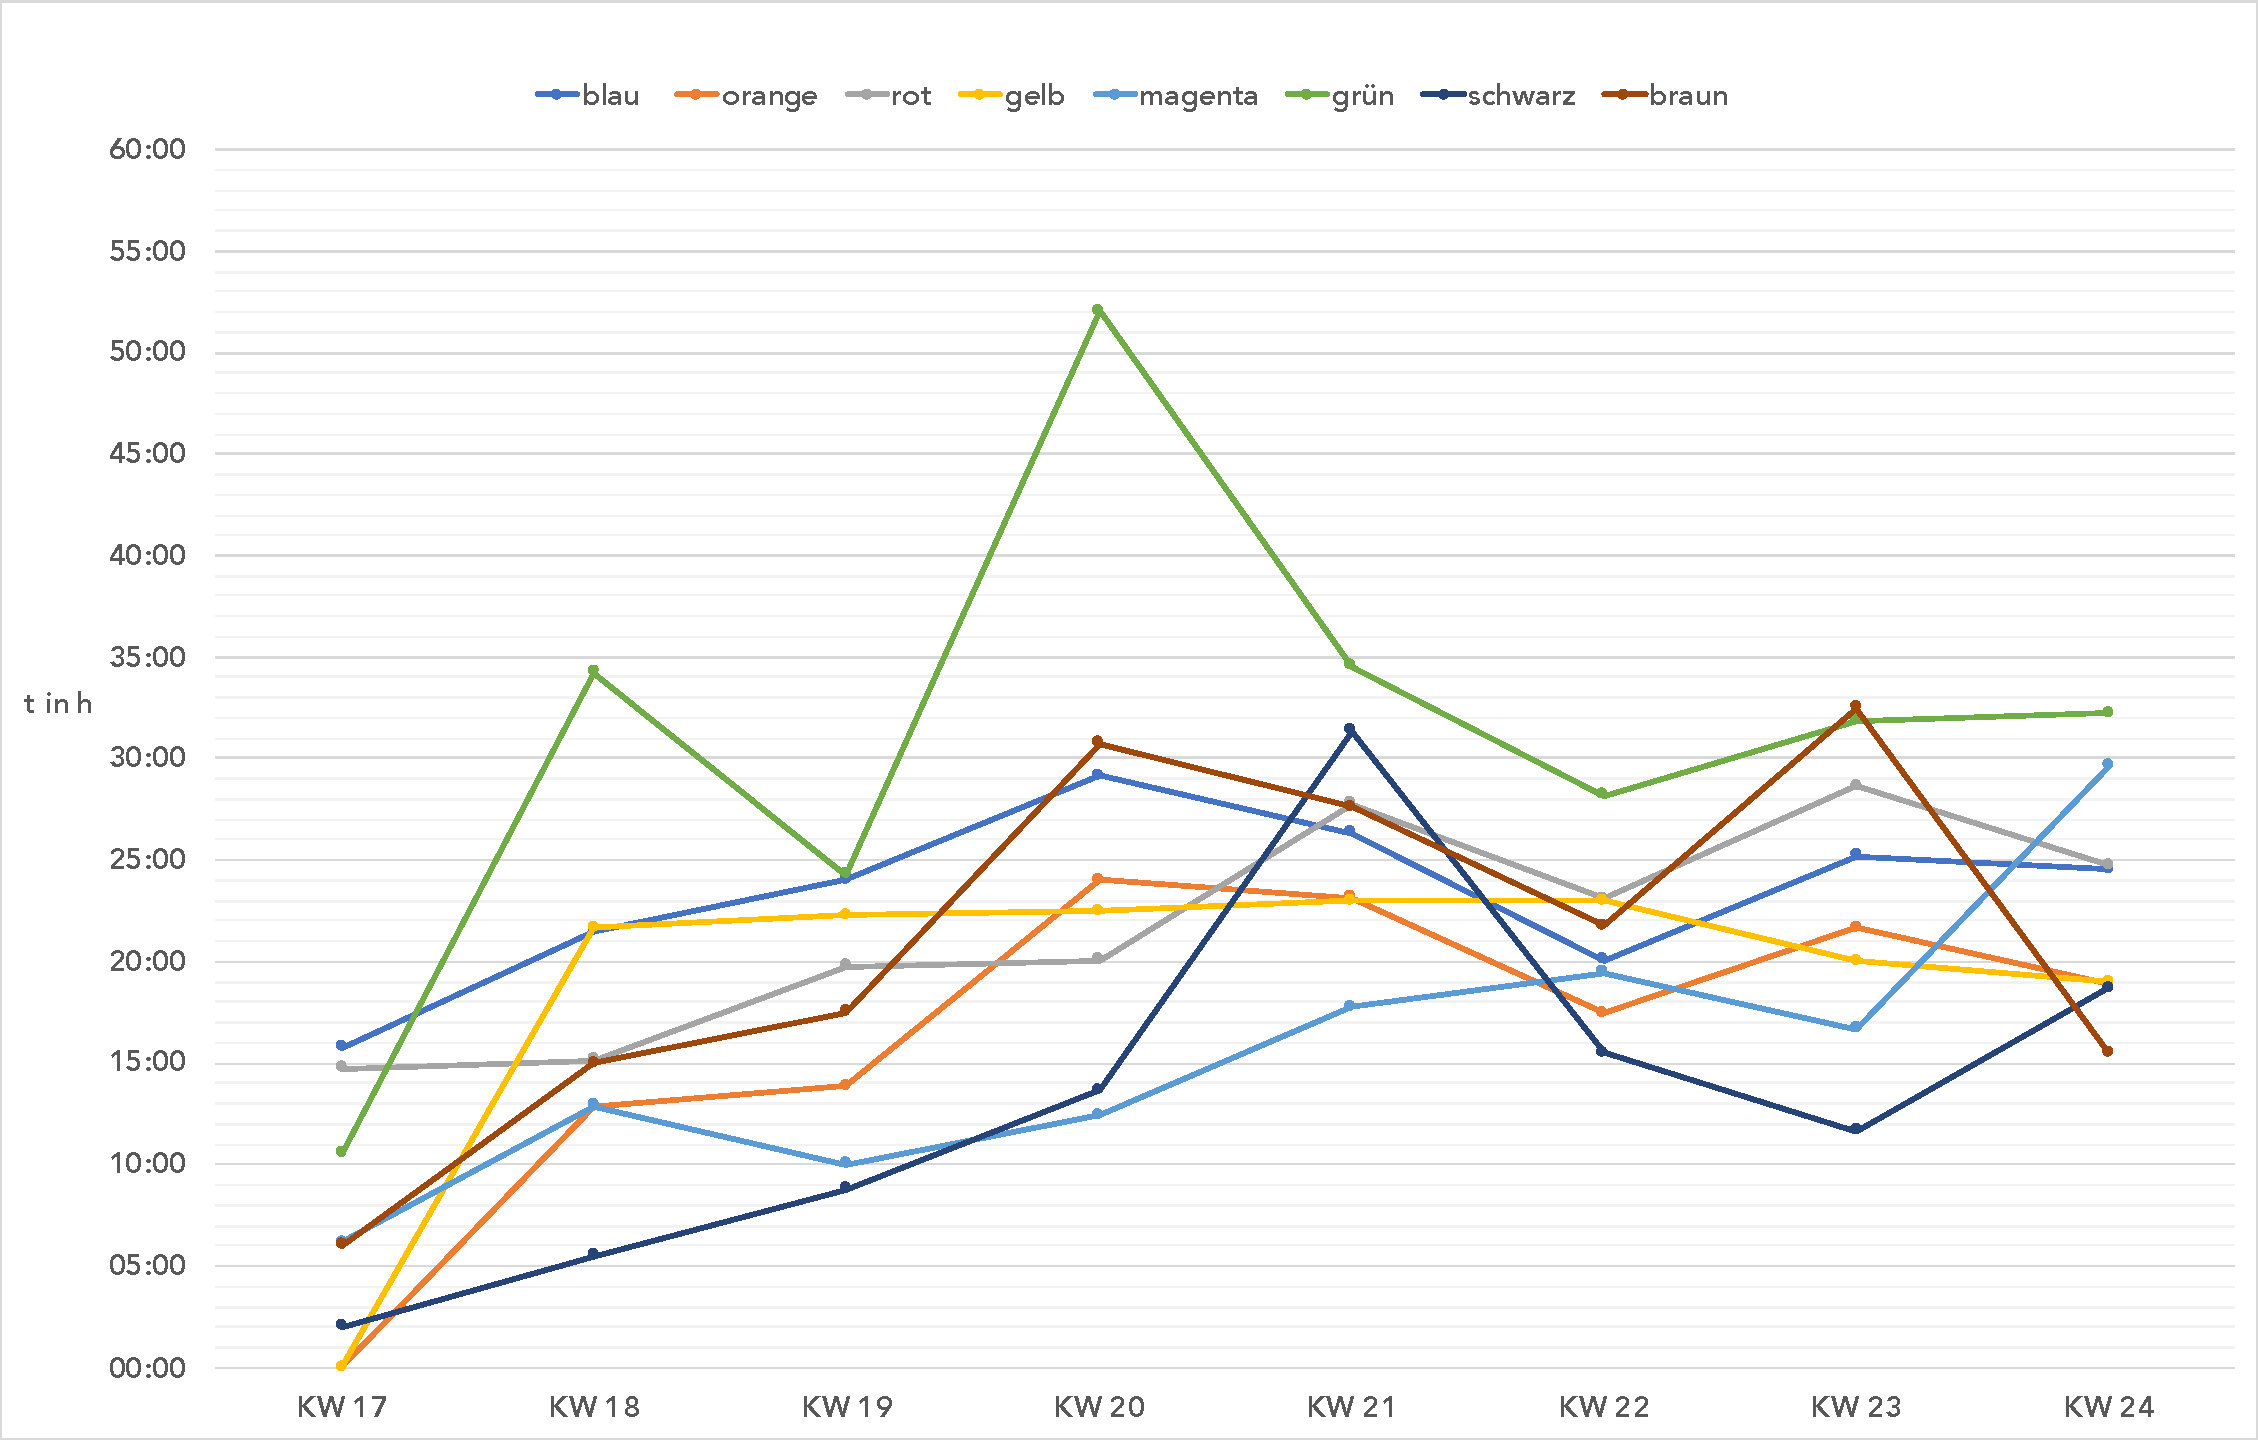
\includegraphics[width = \linewidth]{img/kimai10.pdf}
    \caption{Planungs- und Entwurfsphase und Implementierungsphase (KW 17-24): Zeitaufwand der einzelnen Teammitglieder}
    \label{kimai10}
\end{figure} 

Die Abbildung \ref{kimai10} zeigt den Zeitaufwand der einzelnen Teammitglieder in den Kalenderwochen 17 bis 24. In den Kalenderwochen 17 bis 21 (Planungs- und Entwurfsphase) ist grundsätzlich ein Anstieg bei den meisten Teammitgliedern zu sehen. In den folgenden Wochen (Implementierungsphase) ist dieser nicht mehr so stark zu erkennen. Auch nimmt in den Kalenderwochen 22 bis 24 der Abstand zwischen den einzelnen Punkte in der Abb. \ref{kimai10} ab. Das heißt, dass der Zeitaufwand der einzelnen Teammitglieder sich nicht mehr so stark unterscheidet wie das zum Beispiel in KW 20 der Fall ist. So liegt etwa die Spannweite in KW 20 bei über 39h, während in KW 22 diese bei unter 13h liegt.
\begin{align*}
    R_{KW20} = 52h\: 1min - 12h\: 25min = 39h\: 36min 
\end{align*}
\begin{align*}
   R_{KW22} = 28h\: 10min - 15h\: 19min = 12h\: 51min
\end{align*}
Der maximale Wert an Wochenstunden pro Person bleibt in KW 20 mit über 52h (vgl. Abb. \ref{kimai12}).

\begin{figure} [h]
    \centering
    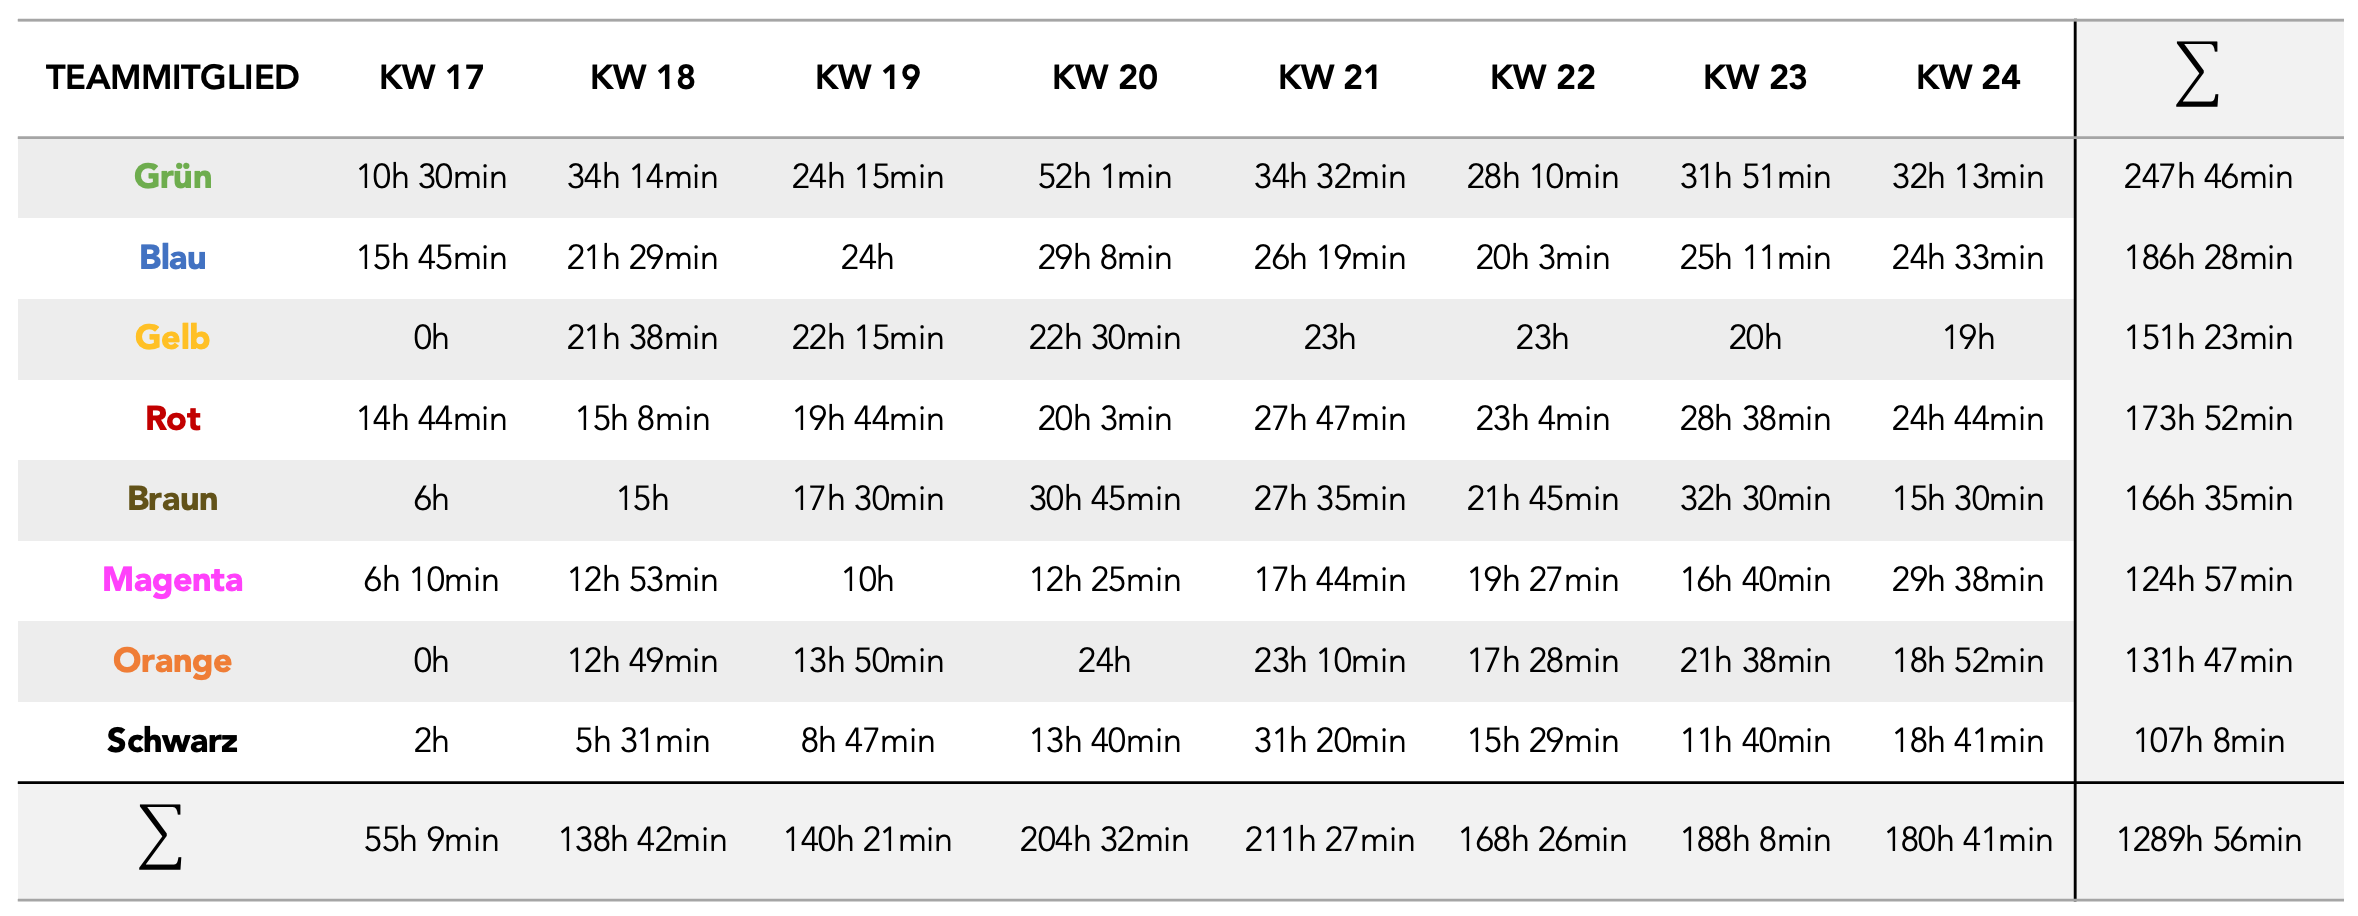
\includegraphics[width = \linewidth]{img/kimai12.png}
    \caption{Planungs- und Entwurfsphase und Implementierungsphase (KW 17-24): Tabelle mit den erfassten Zeiten}
    \label{kimai12}
\end{figure} 
\end{document}
